\documentclass[11pts]{article}
\usepackage[11pt]{moresize}
\usepackage{amsmath}
\usepackage{mathtools}
\usepackage{nccmath}
\usepackage{graphicx}
\begin{document}
	
	

{\HUGE Q 109: Find the vector equation of the line passing through the point 	
	$\begin{psmallmatrix}
		1 \\ 
		2 \\
		-4
	\end{psmallmatrix}$
	and perpendicular to the two lines

$\frac{x-8}{3} = \frac{y+19}{-16}= \frac{z-10}{7} $ and\\\\
$\frac{x-15}{3} = \frac{y-29}{8}= \frac{z-5}{5} $\\

Sol: The vector perpendicular to the 2 lines can be calculated by taking the cross-product of lines.\\
$a = \begin{vmatrix}i & j & k\\ 3 & -16 & 7\\ 3 & 8 & -5\end{vmatrix} $\\
$ = i(-16*(-5) - 8*7) - j (3*(-5) - 3*7) + k(3*8  - (-16)*3)$\\
$ = 24i + 36j + 72k$\\

It passes through (1 2 -4) so the equation of  vector is\\
$ (i + 2j - 4k) + L (24i + 36j + 72k)$ ,where L is any constant\\

\begin{figure*}[hb]
	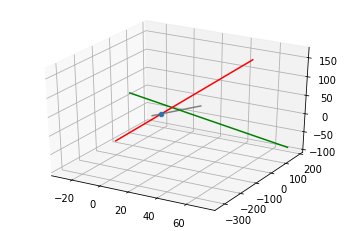
\includegraphics[width=\linewidth]{assignment1.png}
	\caption{perpendicular}
	\label{fig:1}
\end{figure*}
\end{document}